
%%%%%%%%%%%%%%%%%%%%%%% file typeinst.tex %%%%%%%%%%%%%%%%%%%%%%%%%
%
% This is the LaTeX source for the instructions to authors using
% the LaTeX document class 'llncs.cls' for contributions to
% the Lecture Notes in Computer Sciences series.
% http://www.springer.com/lncs       Springer Heidelberg 2006/05/04
%
% It may be used as a template for your own input - copy it
% to a new file with a new name and use it as the basis
% for your article.
%
% NB: the document class 'llncs' has its own and detailed documentation, see
% ftp://ftp.springer.de/data/pubftp/pub/tex/latex/llncs/latex2e/llncsdoc.pdf
%
%%%%%%%%%%%%%%%%%%%%%%%%%%%%%%%%%%%%%%%%%%%%%%%%%%%%%%%%%%%%%%%%%%%


\documentclass[runningheads,a4paper]{llncs}

\usepackage{amssymb}
\usepackage{amsmath}
\setcounter{tocdepth}{3}
\usepackage{graphicx}
\newtheorem{mydef}{Definition}
\newtheorem{mylemma}{Lemma}
\usepackage{algorithm}
\usepackage{tabularx}

\usepackage[noend]{algpseudocode}


\usepackage{url}
\urldef{\mailsa}\path|{jayg, cmhill, mpop}@cs.umd.edu|    
\newcommand{\keywords}[1]{\par\addvspace\baselineskip
\noindent\keywordname\enspace\ignorespaces#1}

\begin{document}

\mainmatter  % start of an individual contribution

% first the title is needed
\title{Identifying Inter-Genomic Repeats Using Fast, Approximate Methods for Betweenness Centrality}

% a short form should be given in case it is too long for the running head
\titlerunning{Inter-Genomic Repeats Using Betweenness Centrality}

% the name(s) of the author(s) follow(s) next
%
% NB: Chinese authors should write their first names(s) in front of
% their surnames. This ensures that the names appear correctly in
% the running heads and the author index.
%
\author{Jay Ghurye%
\and Christopher M. Hill\and Mihai Pop}
%
\authorrunning{Ghurye et al.}
% (feature abused for this document to repeat the title also on left hand pages)

% the affiliations are given next; don't give your e-mail address
% unless you accept that it will be published
\institute{University of Maryland, College Park\\
\mailsa\\}

%
% NB: a more complex sample for affiliations and the mapping to the
% corresponding authors can be found in the file "llncs.dem"
% (search for the string "\mainmatter" where a contribution starts).
% "llncs.dem" accompanies the document class "llncs.cls".
%

\toctitle{Lecture Notes in Computer Science}
\tocauthor{Authors' Instructions}
\maketitle


\begin{abstract}
Assembling metagenomic data is a challenging task due to several reasons. One of the reasons that complicates assembly is the sequences shared between the genomes of multiple organisms. Such regions in genomes are called repeats. Repeats make assembly difficult because they link the unrelated sections of genomes. It has been shown that the number of reconstructions of genome grows exponentially with repeats. Existing approaches to identify repeats are inefficient and do not scale well as size of data increases. We propose an application of a core concept in social network analysis called betweenness centrality to metagenomic data to identify inter-genomic repeats. We show how approximation algorithms for betweenness centrality can be useful to design a faster approach to identify inter-genomic repeats accurately. 
\keywords{Metagenomics, Algorithms, Centrality, Graph}
\end{abstract}


\section{Introduction}

The assembly of metagenomics data, the sequences of DNA recovered from an environment without culturing, is considerably more complex than that of individual genomes.
%Challenges include: (i) repetitive sequences within individual genomes; (ii) varying abundances of different organisms in the community; (iii) variation between closely related organisms; and (iv) conserved genomic segments shared by distantly related organisms.
Repetitive sequences pose a major challenge when assembling isolated genomes.
It has been shown that the number of reconstructions grow exponentially with the number of repeats making it computationally infeasible to find one correct solution for assembly\cite{kingsford}.
The effect of repeats on assembly is exacerbated in metagenomic data sets due to the presence of conserved regions of the genome linking together distantly related organisms.
To tackle the problem of identifying these inter-genomic repeats, several assemblers have used the notion of network centrality to find repeats within the assembly graph.
For example, Bambus2\cite{bambus} uses betweenness centrality to find \emph{central} nodes in the graph.
The drawback of their approach is the expensive calculation of betweenness centrality by computing all-pair shortest paths.
This computation is impractical when applied to the large assembly graphs typically encountered.
To overcome this drawback, we explore the application of approximate and parallel betweenness centrality algorithms on metagenomic assembly graphs and evaluate their effectiveness in identifying inter-genomic repeats.

\section{Related Work}

\subsection*{Betweenness Centrality}
In graph theory and network analysis, indicators of centrality identify the most important vertices within a graph. Several metrics to measure centrality have been proposed. We make use of betweenness centrality. For a particular node, betweenness centrality is equal to the number of shortest paths from all vertices to all others that pass through that node. Formally, for a node $v$, it is defined by following expression:

$$g(v) = \sum_{s \neq t \neq v} \frac{\sigma_{st}(v)}{\sigma_{st}}$$

where $\sigma_{st}$ is the total number of shortest paths from node $s$ to node $t$ and $\sigma_{st}(v)$ is the number of those paths passing through $v$.

Brandes\cite{brandes} gives an exact algorithm for computing betweenness centrality of all the nodes that is based on solving a single source shortest path (SSSP) problem for each node. An SSSP computation from $s$ produces a directed acyclic graph (DAG) encoding all shortest paths starting at $s$.   The contributions of these paths to the betweenness counters can be computed in linear time using backward aggregation. Brandes algorithm calculates $\sigma_{st}$  simultaneously with shortest path calculations: $\sigma_{ss} = 1$ and for $s \neq t, \sigma_{st} = \sum_{v \in pred(t)} \sigma_{sv}$ where $pred(t)$ is a collection of the immediate predecessors of  $t$ on every shortes path ending at $t$. In a subsequent aggregation phase, nodes are procesed by non-decreasing distance from $s$. So we have: 
$$\delta_{s}(v) = \sum_{w \in succ(v)} \frac{\sigma_{sv}}{\sigma_{sw}}(1+\delta_{s}(w))$$

where $\delta_{s}(v) = \frac{\sigma_{st}(v)}{\sigma_{st}}$ and $succ(v)$ is an immediate successor of $v$  in the shortest path DAG.   
This algorithm takes time $\Theta(mn)$ for unit edge weight graphs and $\Theta(mn + n^{2}log(n))$ for weighted graphs. This algorithm does not scale well with large networks with millions of nodes and edges. Bader and Madduri\cite{bader} provide a massively parallel implementation of the exact algorithm. However this approach scales to about a few million nodes and may not be fast enough for larger assembly graphs. 

\subsection*{Betweenness Centrality Based on Sampling Nodes}
Due to scalability limitations of exact betweenness centrality, several approximation algorithms for betweenness centrality have been proposed. Bader and Pich\cite{bp} provide an approximation algorithm by choosing a subset of $k$ starting nodes called pivots and using same aggregation strategy as Brandes algorithm. However, this algorithm overestimates the centrality of some unimportant nodes which are nearer to pivots. The approximation algorithm proposed by Geisberger et al. \cite{sanders} overcomes this drawback by changing the scheme for aggregating betweenness contributions so that nodes nearer to pivots are not unduly profited. The algorithm starts with the sample of $k$ nodes from $|V| = n$ nodes in graph. In each iteration, it chooses one of $2n$ shortest path at random. Here there are $2n$ sample shortest paths because algorithm can do forward search from $s \in V$ or backward search from $t \in V$ and each $s$ and $t$ can have $n$ values. Let $\delta_{P}(v)$ be the contribution received by node $v$ due to shortest path $P$. It can be shown that \cite{sanders} due to all shortest paths $P$ on which $v$ lies, $v$ receives contribution 

$$\delta(v) := \delta_{s}(v) := \sum_{t \in V}\sum \{\delta_{P}(v):  P \in SP_{st}(v)\}$$
due to a forward search, and 

$$\delta(v) := \delta_{t}(v) := \sum_{s \in V}\sum \{\delta_{P}(v):  P \in SP_{st}(v)\}$$
due to a backward search. 

This algorithm is efficiently implemented by modifying original aggregation scheme of Brandes algorithm so that the nodes near the sampled node will not receive high centrality score. Runtime of the algorithm largely depends on the size of the sample we choose. However,there is a tradeoff between size of sample and accuracy of centrality detection.  



\begin{figure*}[htbp]
\centering
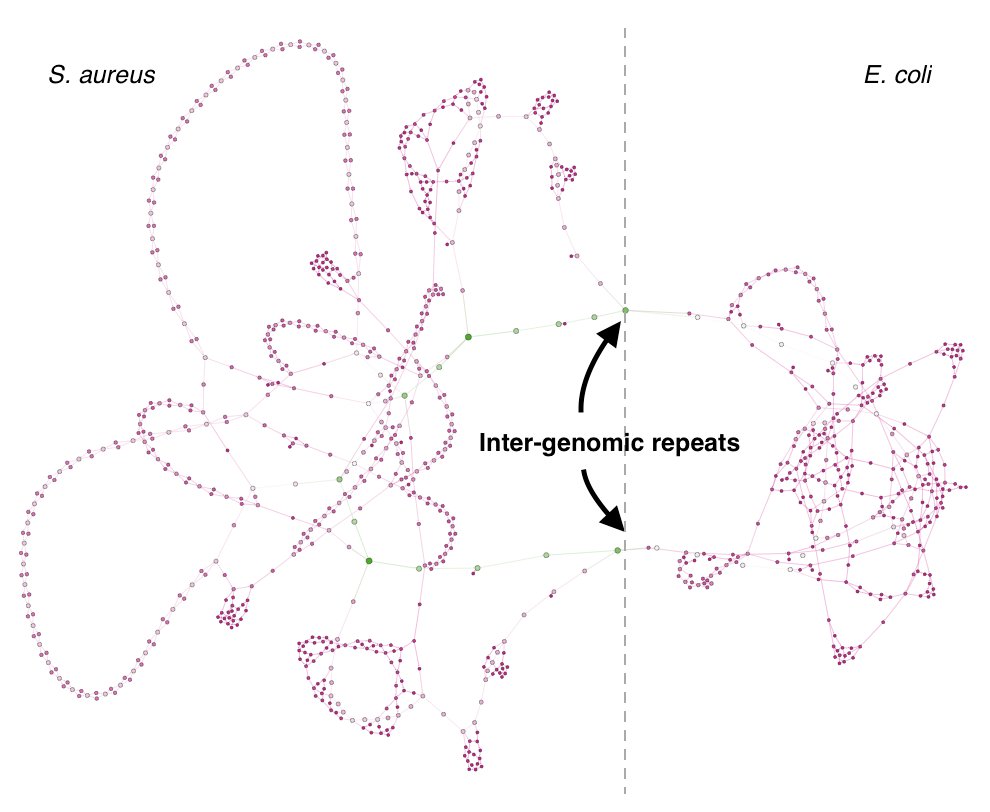
\includegraphics[width=0.60\textwidth]{es_mix_200kb_k21.png}
\caption{Assembly graph of a simulated community consisting of 200 Kbp subsets of \textit{Escherichia coli} str. K-12 MG1655 and \textit{Staphylococcus aureus}.  Nodes are colored and sized based on their relative betweenness centrality. The highlighted nodes are inter-genomic repeats whose deletion would separate the graph. Note that the betweenness centrality measure correctly identifies these nodes.}
\label{fig:sampled_nodes}
\end{figure*}


\subsection*{Betweenness Centrality Based on Sampling Shortest Paths}
Another approximation algorithm was proposed by Matteo et al. \cite{matteo} based on randomized sampling of shortest paths and offer probabilistic guarantees on the quality of approximation. This algorithm guarantees that all approximate values of betweenness for all vertices are within an additive factor $\epsilon \in (0,1)$ from the real values with probability at least $1-\delta$. To derive bounds on sample size, results from VC dimension theory\cite{vc} are used. The main advantage of this algorithm is that the sample size does not depend on the size of the graph, but only on the maximum number vertices in a shortest path which is called \textit{vertex diameter}. The sample size $r$ of shortest paths is found out with the help of $VD(G)$ as follows:
\begin{equation} \label{sample_size_algo}
r = \frac{c}{\epsilon^{2}}(\left\lfloor{log_{2}(VD(G) - 2)}\right\rfloor + 1 + ln\frac{1}{\delta})
\end{equation} 
where $c$ is a constant with value $0.5$. 

The algorithm estimates the vertex diameter of the graph using a simple $2-$approximation algorithm. The shortest paths are sampled using weighted random sampling. The runtime of this algorithm is dominated by the computation of shortest path at each step which takes time $O(|V| + |E|)$ for unweighted graphs(BFS) and $O(|E| + |V|log|V|)$ otherwise (Dijkstra's algorithm). This is multiplied by $r$ for $r$ iterations to obtain final complexity.


\section{Methods}


\subsection*{Simulating Metagenomic Assembly Repeat Graphs}

We evaluate the efficacy of detecting inter-genomic repeats using the approximate betweenness centrality methods on simulated metagenomic assembly graphs.
The first step is to construct the \textit{de Bruijn} graph from the set of reference genomes.
De Bruijn strings are a type of ``comprehensive'' strings. For a given alphabet $\Sigma = \{A,C,T,G\}$ and a length $k$, a de Bruijn string of order $k$ contains as substrings of length $k$ over $\Sigma$. These strings can be represented in a sophisticated way in term of a graph called de Bruijn graph \cite{debruijn}. A de Bruijn graph of order $k$ is a graph that contains all strings of length $k-1$ from a given alphabets as nodes and contains edges between two nodes if the corresponding strings overlap by exactly $k-2$ letters in prefix-suffix manner. In other words, each $k$-mer is represented by two nodes in a graph connected by an edge. 

Next we modify the de Bruijn graph generated from genomes to identify repeats. We define \textit{unipaths} as the path of nodes in which the outdegree of first node on the path is $1$ and indegree is not equal to $1$, indegree of last node on the path is $1$ and outdegree is not equal to $1$ and for all other nodes along the path, both indegree and out degree is exactly $1$. We compress all the unipaths in a graph to represent the path in a compact way. We represent the unipath as a single node whose label is the concatenation of all node labels along the path.
Nodes in the resulting graph represent uniquely resolvable sequences of length $\geq k$.

For evaluation we simulate metagenomic assembly graphs consisting of two, five, and ten bacterial genomes.
The composition of each simulated sample is described in Table \ref{tab:composition}.
For the five and ten metagenome samples, random bacterial genomes were chosen from the data set provided by \cite{shakya2013comparative}.
A $k$-mer size of 55 was chosen for initial creation of the de Bruijn graph.

\begin{table}[h]
\centering
\caption[]{Composition of simulated metagenomic assembly graph.}
\begin{tabularx}{\linewidth}{|l|X|l|l|}
\hline
\textbf{Name} & \textbf{Genomes} & \textbf{Nodes} & \textbf{Edges} \\
\hline
2-genome & \textit{Escherichia coli} str. K-12, \textit{Staphylococcus aureus}  & 3,384 & 4,534 \\
\hline
5-genome & \textit{Burkholderia xenovorans} LB400, \textit{Archaeoglobus fulgidus} DSM 4304,  \textit{Pyrobaculum calidifontis} JCM 11548, \textit{Zymomonas mobilis subsp. mobilis} ZM4, \textit{Porphyromonas gingivalis} ATCC 33277 & 5,114 & 6,844  \\
\hline
10-genome  & \textit{Caldicellulosiruptor bescii} DSM 6725, \textit{Bacteroides vulgatus} ATCC 8482, 
 \textit{Bacteroides thetaiotaomicron} VPI-5482, \textit{Clostridium thermocellum} ATCC 27405, 
 \textit{Pyrobaculum arsenaticum} DSM 13514, \textit{Chlorobium phaeobacteroides} DSM 266, 
 \textit{Ruegeria pomeroyi} DSS-3, \textit{Treponema denticola} ATCC 35405, 
 \textit{Porphyromonas gingivalis} ATCC 33277, \textit{Nostoc sp.} PCC 7120  & 25,425 & 34,056\\
\hline 
\end{tabularx}
\label{tab:composition}
\end{table}

Apart from simulated metagenomic graphs, we study how approximation algorithms for betweenness centrality work on real datasets. We evaluated the runtime  of these algorithms on metagenomic stool sample of a premature infant\cite{morowitz2011strain}. This graph has 3797425 nodes and 2970379 edges. We compared the performance of Bambus2's repeat detection module on this data with the performance of approximate betweenness centrality algorithms.  

\subsection*{Evaluation}
We evaluate the effect of using approximation algorithms for betweenness centrality on finding inter-genome repeats using the simulated datasets described above.
%We use the notion of Sensitivity, specificity, and precision to define the quality of repeat detection.
A good repeat detection strategy should have high sensitivity, specificity, and precision. Sensitivity is the measure of proportion of actual repeats which are correctly identified by the algorithm. Specificity is the proportion of non-repeats correctly identified by the algorithm. Precision is the proportion of repeats identified that are correct. High sensitivity is desired because we want to remove as many repeats from the graph. High specificity is desired because we do not want to remove non-repeats which are incorrectly identified as repeats by algorithm. High precision helps us determine the usefulness of our methods. To calculate sensitivity, specificity, and precision, we define following terms:
\begin{itemize}
\item \textbf{True positives(TP):} Number of nodes marked as a repeat that is found within at least 2 genomes
\item \textbf{False positives(FP):} Number of nodes marked as a repeat that is only found within a single genome
\item \textbf{True negatives(TN):} Number of nodes marked as a non-repeat that is only found within a single genome
\item \textbf{False negatives(FN):} Number of nodes marked as a non-repeat that is found within at least 2 genomes
\end{itemize}

Using these quantities, we can define sensitivity and specificity as follows:
 $$Sensitivity = \frac{TP}{TP+FN}$$
 $$Specificity = \frac{TN}{TN+FP}$$
 $$Precision = \frac{TP}{TP + FP}$$

For evaluating the effect of node sampling on inter-genomic repeat detection, we sample between 10 to 10,000 nodes per trial.
For evaluating path sampling, we select epsilon parameters between 0.01 and 0.20.
The result of each parameter is averaged over 10 trials.


\subsection*{Cutoff Criteria For Repeats}
Bambus2\cite{bambus} uses exact betweenness centrality to find repeats. To filter out repeats, it calculates mean $\mu$ and standard deviation $\sigma$ over the centrality scores for all the nodes in graph. It then marks all the nodes with centrality score greater than $\mu + 3*\sigma$ as repeats. To filter out repeats based on approximate centrality scores, we use the same method as Bambus2. 

Another cutoff criteria we test is based on \textit{interquartile range(IQR)}. Let $Q_{1}$,$Q_{2}$, and $Q_{3}$ denote the lower, middle and upper quartiles respectively. IQR can be defined as the difference between the upper and lower quartile. So, $IQR = Q_{3} - Q_{1}$. For the values of centrality, we calculate upper quartile, middle quartile, lower quartile and IQR. For filtering, we mark all the nodes with centrality more than $Q_{3} + 1.5*IQR$ as repeats. The advantage of this method is that it does not make any assumptions about the distribution of underlying data. 

\subsection*{Implementation}
We investigate the performance of approximate betweenness centrality algorithms on the metagenomic graphs to find inter-genome repeats. We carried out experiments on a 64-bit Linux machine with 12 CPUs and 50 GB memory. We used the implementations provided by \textsc{NetworKit}\cite{networkit} library. It implements effecient graph algorithms and parallelize most of them. It provides implementation for variety of centrality measures. We used the implementation of approximate betweenness centrality. For our experiments, we use the parallelized implementation for the algorithm by Matteo et al.\cite{matteo} and serial implementation for the algorithm by Geisberger et al.\cite{sanders}.


\section{Results} 


\subsection*{Approximate Betweenness Centrality Retains Detection Power of Inter-Genomic Repeats}

Across all data sets, the more nodes and paths sampled, the better the inter-genomic repeat detection (Figures \ref{fig:sampled_nodes} and \ref{fig:sampled_paths}).
Furthermore, the runtime increases linearly with the number of nodes sampled (Figure \ref{fig:sampled_nodes}).
In the 2-genome assembly graph, all inter-genomic repeats were found by sampling as few as ten nodes, an order of magnitude less time than calculating the betweenness centrality using the full graph.
In the 5-genome assembly graph, sampling 10 nodes has a sensitivity of 86\% and reaches 100\% at 500 nodes which is approximately one-tenth the size of the assembly graph.
The sensitivity drops off drastically in the 10-genome assembly graph, oscillating around 6\% across all node sample sizes.
While the specificity remains consistent across data sets (97\%-99\%), the precision increases from ~2.5\% to ~25\% when going from the 2-genome to the 10-genome data set.

For the range of epsilon parameters used, the statistical measures of repeat detection remain constant (Figure \ref{fig:sampled_paths}).
Similarly, the runtime for each epsilon parameter remains relatively unchanged except for a slight change in the 10-genome sample.
For the 10-genome sample, the statistical measures and runtime are equivalent to when 100-500 nodes are sampled.

\begin{figure}[htbp]
\centering
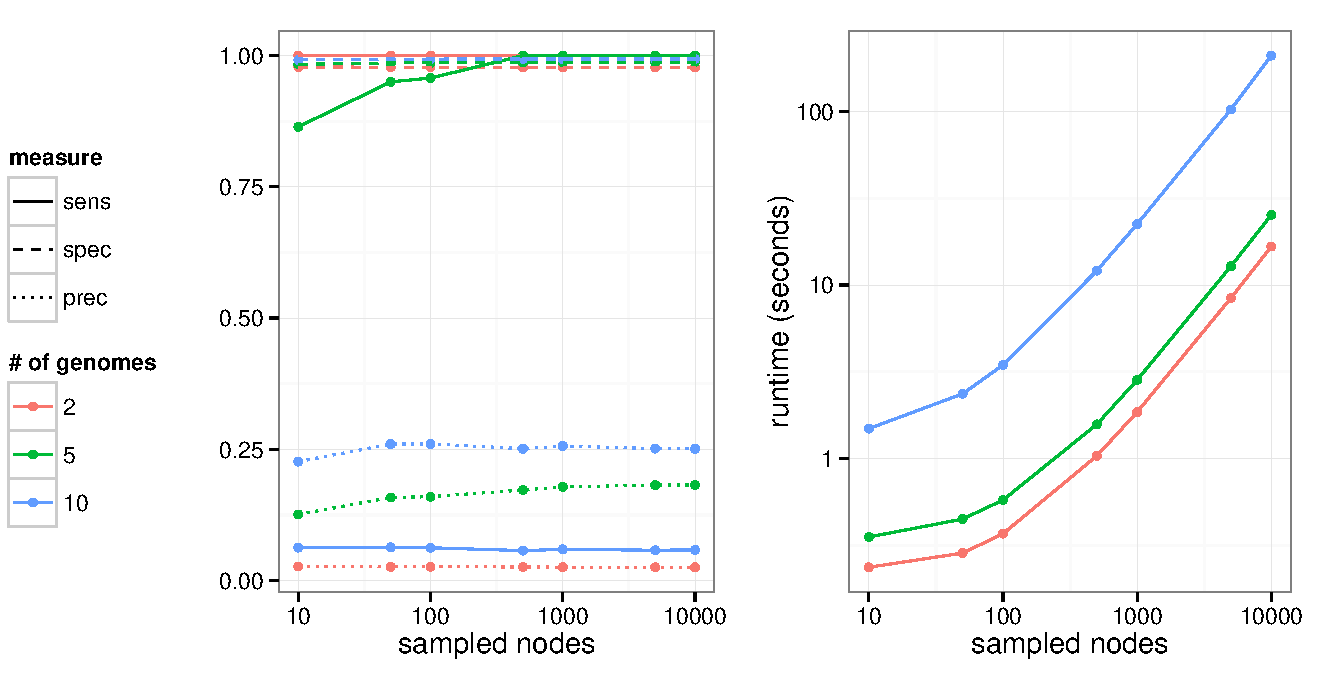
\includegraphics[width = \textwidth]{sampled_nodes}
\caption{Statistical measures of repeat detection quality for the simulated metagenomic assembly graphs. Betweenness centrality was approximated by randomly sampling nodes in the graph.}
\label{fig:sampled_nodes}
\end{figure}

\begin{figure}[htbp]
\centering
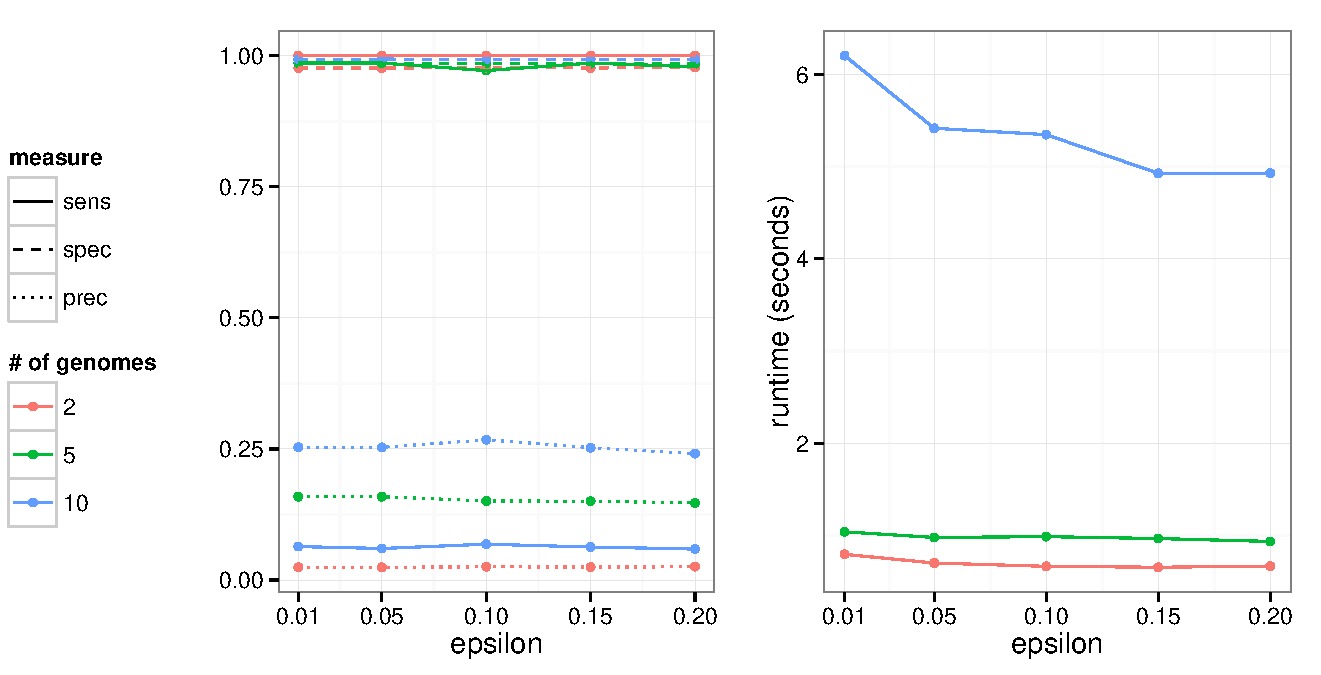
\includegraphics[width = \textwidth]{sampled_paths}
\caption{Statistical measures of repeat detection quality for the simulated metagenomic assembly graphs. Betweenness centrality was approximated within epsilon of their true value.}
\label{fig:sampled_paths}
\end{figure}

\subsection*{Alternate Betweenness Centrality Cutoff Increases Sensitivity}

Decreasing the betweenness centrality cutoff requirement results in a trade-off between the different statistical measures.
Instead of using the default cutoff of $3\sigma$ suggested by Bambus2, we mark all the nodes with centrality more than $Q_{3} + 1.5*IQR$ as an inter-genomic repeats.
In the 10-genome assembly graph, the sensitivity increases from 5.8\% to 34.4\% when using the IQR cutoff method.
Conversely, the specificity and and precision drops from 99.3\% to 90.9\% and 25\% to 12.5\%, respectively.


\subsection*{Results On Real Metagenomic Datasets}
We evaluated the performance of approximate betweenness centrality algorithms on metagenomic stool sample. We compared the performance of these algorithms with Bambus2 repeat detection module. Bambus2 repeat detection module took over 50 hours to find repeats in this graph. The algorithm based on sampling shortest paths took 312.69 seconds for $\epsilon = 0.1$ to find out repeats. The algorithm based on sampling nodes took 469 seconds for the sample of 1000 nodes and around 5000 seconds(1.3 hours) for the sample of 10000 nodes. From these results it can be concluded that we can use approximation algorithms for repeat finding and get significant speedups.  


\section{Discussion}
Betweenness centrality is a proven method for finding inter-genomic repeats in metagenomic assemblies.
The size of typical metagenomic assembly graphs often make it infeasible to calculate the exact betweenness centrality of each node.
We have taken the first steps to show how recent approximation algorithms for calculating betweenness centrality can be used retain the same repeat detection power as the exact algorithms in a fraction of the time.
In the future, larger and more complex metagenomic assembly graphs must be used to further evaluate the efficacy of the approximation algorithms.

\section{Conclusion}
In this work, we show how approximate betweenness centrality can be used to identify inter-genome repeats. We explored two algorithms, one based on sampling shortest paths in a graph and other based on sampling nodes in a graph. Application of both these algorithms to repeat detection problem provided accurate and fast results. We explore how various parameters such as number of sampled nodes and filtering criteria to mark a node as repeat affects the accuracy of repeat detection. We are planning to use these techniques for repeat detection in our future metagenomic assembler. 
\bibliography{manuscript}{}
\bibliographystyle{abbrv}

\end{document}
